\chapter{Studi Eksplorasi}
\label{chap:Eksplorasi}

Pada Bab ini akan dibahas Konfigurasi Spark, Twitter API, dan Kafka pada perangkat dengan sistem operasi windows. Selain itu, pada bab ini akan dijelaskan contoh eksekusi program Spark Streaming pada TCP Socket dan Twitter API. Serta, mengambil data dari Kafka.

\section{Konfigurasi Klaster}

\subsection{Konfigurasi Hadoop}
Hadoop merupakan framework yang dibuat untuk berjalan pada sistem operasi berbasis Linux,
sehingga versi-versi awal Hadoop tidak dapat digunakan untuk sistem operasi Windows. Penggunaan
Hadoop untuk Windows dapat dilakukan mulai Hadoop versi 2.x dengan menggunakan file-file
tambahan. Sebelum melakukan konfigurasi, berikut ini adalah komponen-komponen yang diperlukan
untuk dapat melakukan konfigurasi dan menjalankan Hadoop pada sistem operasi Windows 10 x64.

\begin{itemize}
	\item Java JDK 8
	\item Paket biner Hadoop versi 3.x.
	\item Paket winutils dengan versi yang sama dengan versi Hadoop yang digunakan
	\item Microsoft Visual C++ 2010 Redistributable
\end{itemize}

Hadoop berjalan dengan menggunakan virtual machine milik Java, sehingga instalasi Java perangkat
diperlukan terlebih dahulu. Berdasarkan gambar 3.1, pengguna disarankan mengganti tempat
instalasi Java yang digunakan dengan mencentang pilihan Change destination folder. Tempat
instalasi awal Java pada umumnya akan berada di \path{C:\Program\Files\Java} atau \path{C:\Program\Files\(x86)\Java}. Hal ini dapat menimbulkan masalah pada Hadoop karena Hadoop tidak
mendukung menggunaan karakter spasi pada nama direktori. Oleh karena itu, direktori tempat
instalasi Java diubah menjadi direktori lain dengan nama yang tidak menggunakan karakter spasi.

\begin{figure}[H] 
	\centering  
	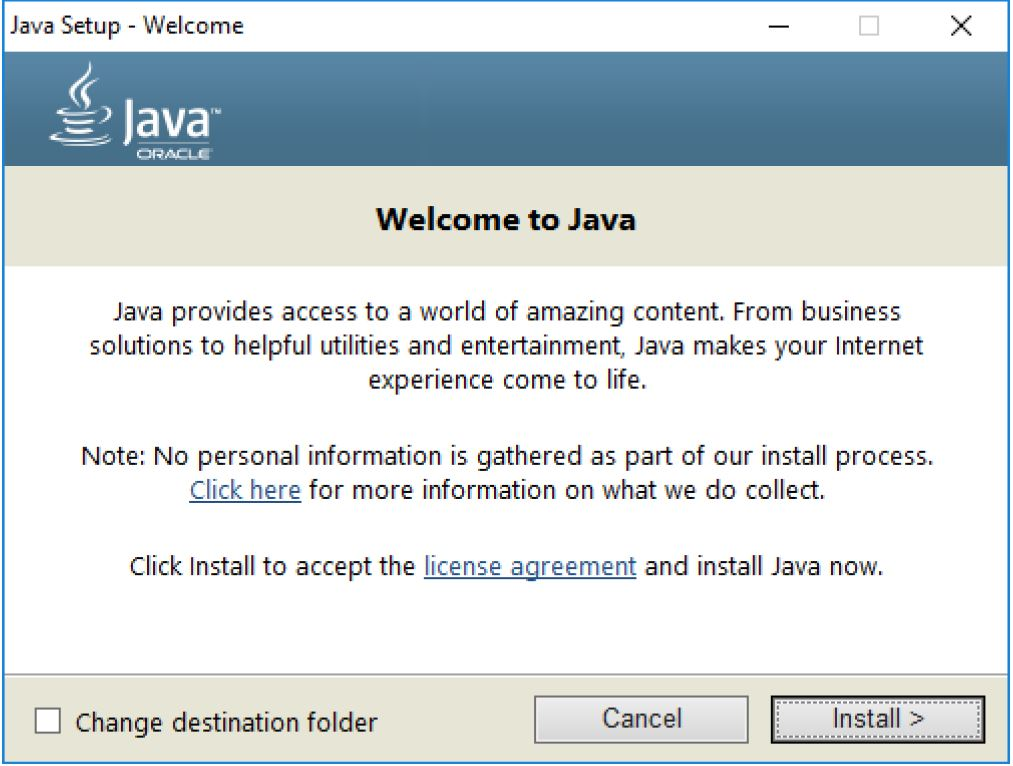
\includegraphics[scale=0.5]{instalasiJava}  
	\caption[Gambar Instalasi Java]{Instalasi Java} 
	\label{fig:Java-instalation} 
\end{figure}
 
Setelah instalasi selesai dilakukan, environment variable untuk JAVA \char`_HOME perlu ditambahkan.
Nilai untuk \textit{environment variable} tersebut merupakan direktori instalasi Java pada perangkat. Seperti yang sudah disebutkan sebelumnya, direktori tersebut disarankan tidak menggunakan karakter spasi sesuai dengan yang ditunjukkan pada gambar 3.2.

\begin{figure}[H] 
	\centering  
	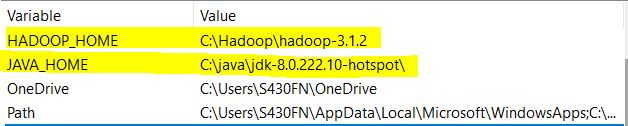
\includegraphics[scale=0.8]{environmentHadoop}  
	\caption[Gambar HADOO PHOME]{\textit{Environment variable} untuk \texttt{JAVA \char`_HOME} dan
	\texttt{HADOOP \char`_HOME}} 
	\label{fig:Hadoop-home} 
\end{figure}

Setelah instalasi dan penambahan environment variable, file-file biner Hadoop dapat diekstraksi
pada sebuah direktori. Direktori tersebut sebaiknya memiliki nama yang cukup ringkas dan
tidak menggunakan karakter spasi. Untuk memudahkan penggunaan Hadoop, alamat direktori
tersebut dapat ditambahkan sebagai environment variable dengan nama HADOOP \char`_HOME seperti yang
ditunjukkan pada gambar 3.2.
Konfigurasi klaster yang perlu dilakukan berupa konfigurasi untuk HDFS dan MapReduce untuk
klaster single node. Konfigurasi tambahan perlu dilakukan pada file masters dan slaves untuk
penggunaan klaster multi node.

Konfigurasi HDFS dilakukan dengan membuat atau mengisi file-file hadoop-env.cmd, core-site.xml,
dan hdfs-site.xml.

\subsection{Konfigurasi Spark}
Klaster yang digunakan Spark pada skripsi ini adalah klaster yang sama dengan Hadoop.Versi
Spark yang digunakan untuk pengembangan aplikasi adalah Spark 2.4.3 dengan sistem operasi Windows 10 x64.Berikut ini adalah langkah-langkah melakukan konfigurasi Spark pada komputer-komputer
bagian klaster. Instalasi Spark hanya mengatur \textit{environment variable} sesuai dengan direktori Spark dan menambah environment ke path. Namun harus terdapat Hadoop yang telah terinstal sebelumnya.
Setelah semua terinstal dan perintah \texttt{Spark-shell --version} dipanggil akan muncul layar seperti ini:

\begin{figure}[H] 
	\centering  
	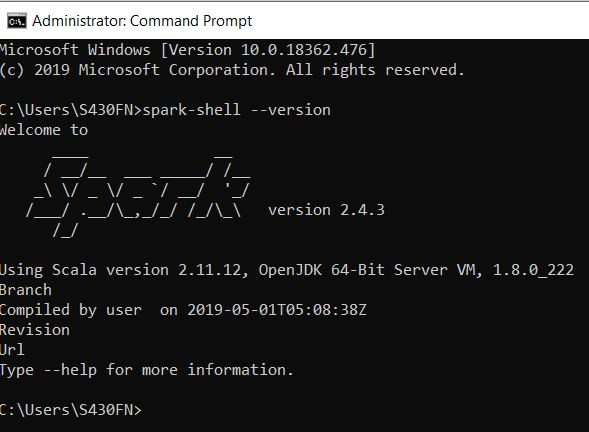
\includegraphics[scale=0.8]{SparkHome}  
	\caption[Gambar Spark]{Gambar Spark berhasil diinstal} 
	\label{fig:Hadoop-home} 
\end{figure}

Jika Spark telah terinstal perintah scala akan langsung bisa dijalankan.

\section{Konfigurasi API dan Data Collector}
Karena data yang dibutuhkan untuk Spark Streaming harus besar dan real-time maka dibutuhkan sistem lain yang terintegrasi sebagai penyedia data. Beberapa contoh sistem tersebut adalah Twitter API dan
Kafka. Twitter API menyediakan data hanya dari twitter saja. Sedangkan, Kafka bisa menerima data hampir dari semua API.

\subsection{Konfigurasi TCP Socket}
Sumber data TCP Socket tidak perlu diinstalasi terlebih dahulu karena tidak ada interverensi dari pihak ketiga yaitu sang penyedia data. TCP socket langsung bisa menerimas data dengan mengakses port lokal dan akan langsung terintegrasi dengan IP address dan port yang kita miliki. Mengkonfigurasikan TCP Socket hanya perlu menyediakan sebuah port kosong yang nantinya akan digunakan data untuk masuk. Tetapi, konfigurasi pada kode program masih diperlukan.


\subsection{Konfigurasi Twitter API}
Sebelum mendapatkan hak untuk mengakses Twitter API, user perlu melakukan pendaftaran ke pihak twitter untuk menjadi \textit{developer account} terlebih dahulu. Akan muncul survei yang menanyakan tentang privasi data pengguna twitter.Pertanyaan paling umum adalah data yang didapatkan akan digunakan untuk apa. Untuk kasus skripsi ini, data akan digunakan untuk mempelajari Spark Streaming. Berikut adalah cara membuat API Setelah dikonfirmasi menjadi \textit{developer account}:

\begin{enumerate}
	\item Membuat Aplikasi yang akan digunakan sebagai API.
	\item Mengisi keterangan dan informasi tentang aplikasi tersebut
	\item Menggunakan keys dan tokens yang didapatkan yang akan digunakan untuk integrasi dengan 			Spark Streaming
\end{enumerate} 

keys dan tokens yang didapatkan adalah beberapa nomer seri yang disbut \textit{Consumer API} dan \textit{Access token}. Nomor seri ini yang nantinya akan jadi parameter bagi kode program untuk mengakses Aplikasi yang telah kita buat. Nomor seri ini bersifat rahasia jadi tidak boleh tersebar ke pihak lain karena seseorang bisa mengakses Aplikasi pengumpul data yang telah kita buat. Berikut contoh gambar dari key dan tokens:

\begin{figure}[H] 
	\centering  
	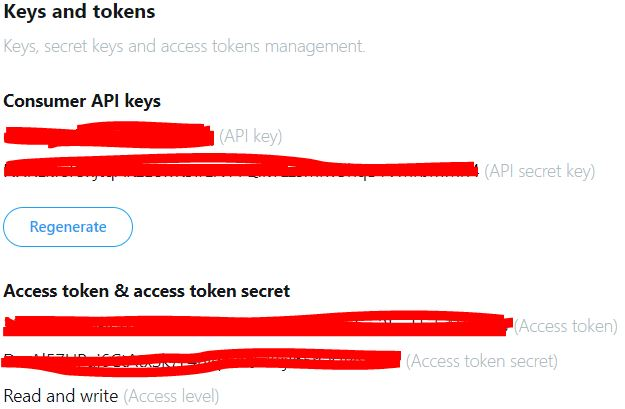
\includegraphics[scale=0.8]{TwitterTokens}  
	\caption[Gambar Twitter Tokens]{Gambar Token yang digunakan sebagai parameter} 
	\label{fig:Hadoop-home} 
\end{figure}

Parameter keys dan token nantinya akan dimuat dalam \texttt{twitterAuth.txt}. File tersebut akan dijadikan sebagai otentikasi untuk mengakses data yang ada di Twitter.
 
\subsection{Konfigurasi Kafka}
kafka adalah sebuah sistem pengriman data \textit{Publish/subscribe} yang didesain untuk menyelesaikan masalah yang sering disebut dengan \textit{distributed commit log} yang mana suatu \textit{filesystem} atau database didesain untuk menyediakan data rekord-rekord yang disimpan dengan lama dan bisa diakses kembali secara berkala pada sistem yang stabil. Kafka akan menjadi Input Sources bagi spark streaming. Sebelum instalasi kafka berikut komponen-komponen yang dibutuhkan untuk menjalankan kafka di windows 10 x64:


\begin{itemize}
	\item Java JDK 8
	\item Zookeeper
	\item Paket winutils dengan versi yang sama dengan versi Hadoop yang digunakan
\end{itemize}

karena zookeeper berjalan di atas java maka sebelum instalasi zookeeper dan kafka harus menginstal java JDK 8.instalasi Java yang digunakan dengan mencentang pilihan \texttt{Change destination folder}. Tempat instalasi awal Java pada umumnya akan berada di \path{C:\Program\Files\Java} atau \path{C:\Program\Files\(x86)\Java}. Hal ini dapat menimbulkan masalah pada Zookeeper karena Zookeeper tidak mendukung menggunaan karakter spasi pada nama direktori. Oleh karena itu, direktori tempat instalasi Java diubah menjadi direktori lain dengan nama yang tidak menggunakan karakter spasi.

\begin{figure}[H] 
	\centering  
	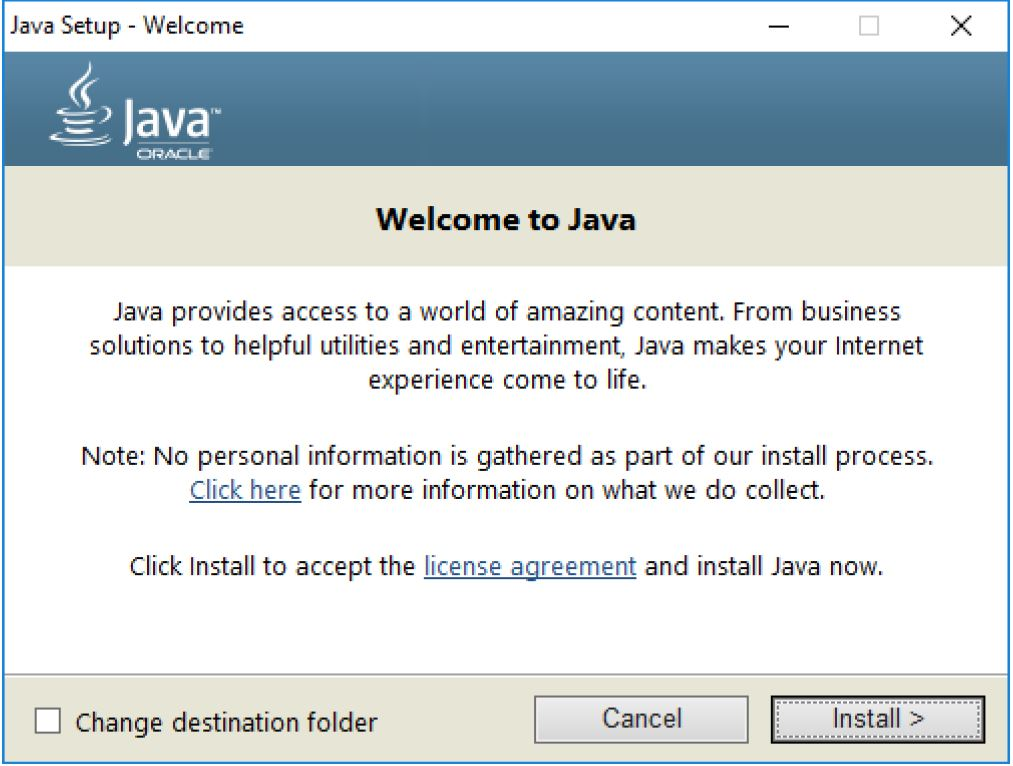
\includegraphics[scale=0.5]{instalasiJava}  
	\caption[Gambar Instalasi Java]{Instalasi Java} 
	\label{fig:Java-instalation} 
\end{figure}

Setelah menginstal java harus menginstal zookeeper terlebih dahulu karena kafka menggunakan zookeeper untuk menyimpan metadata tentang klaster kafka. Zookeeper yang digunakan adalah zookeeper versi $3.5.x$. Lalu, ubahlah konfigurasi pada \texttt{zoo.cfg} dan ubahlah direktori tempat metadata kafka mau disimpan. contoh \path{\zookeeper-3.5.6\data}. setelah itu, \textit{environment variable} untuk ZOOKEEPER \char`_HOME perlu ditambahkan. Nilai untuk \textit{environment variable} tersebut merupakan direktori instalasi ZOOKEEPER pada perangkat. Seperti yang sudah disebutkan sebelumnya, direktori tersebut disarankan tidak menggunakan karakter spasi.sesuai dengan yang ditunjukkan pada gambar 3.2. 

\begin{figure}[H] 
	\centering  
	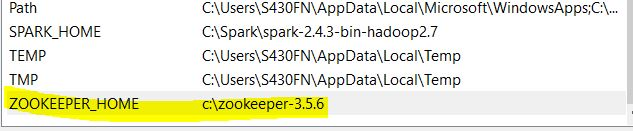
\includegraphics[scale=0.8]{zookeeperhome}  
	\caption[Gambar ZOOKEEPER \char`_HOME]{ZOOKEEPER \char`_HOME} 
	\label{fig:zookeeper-instalation} 
\end{figure}

Untuk sistem \textit{standalone} port zookeper bisa diatur. tetapi port default adalah 2181. Untuk
menjalankan Zookeper lakukan perintah \texttt{zkserver}. Sebelum menginstal broker pastikan zookeeper berjalan terlebih dahulu. Setelah zookeeper berhasil terinstal. perlu menjalankan broker karena \textit{consumer} dan \textit{producer} membutukan \textit{broker} untuk bisa diinstal dan saling berkomunikasi. perintah untuk menjalankan broker: \path{.\bin\windows\kafka-server-start.bat .\config\server.properties}. Setelah menjalankan broker dan zookeeper, membuat \textit{topics} untuk kafka.

\begin{figure}[H] 
	\centering  
	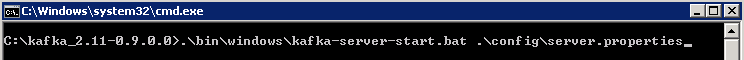
\includegraphics[scale=0.8]{serverkafka}  
	\caption[Gambar menjalankan server]{menjalankan server} 
	\label{fig:topic-run} 
\end{figure}

\textit{Topics} yang dibuat dengan nama \"Test\" dan akan direplika sebanyak satu kali jika \textit{standalone}. Jika memiliki klaster lebih dari satu maka bisa mereplikasi lebih dari satu dan replikasi tersebut digunakan sebagai \textit{backup} jika terjadi kegagalan. Topik dapat dibuat dengan perintah: \path{kafka-topics.bat --create --zookeeper localhost:2181 --replication-factor 1 --partitions 1 --topic test}

\begin{figure}[H] 
	\centering  
	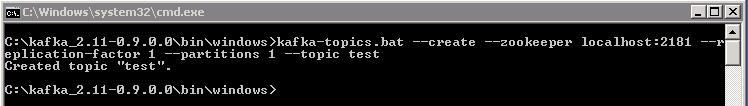
\includegraphics[scale=0.8]{topickafka}  
	\caption[Gambar menjalankan topic]{menjalankan topic} 
	\label{fig:topic-run} 
\end{figure}

Untuk mengetes apakah suatu server sudah jalan perlu dilakukan pengecekan dengan membuat broker \textit{producer} dan \textit{consumer}. Untuk menjalankan \textit{producer}, lakukan perintah \path{kafka-console-producer.bat --broker-list localhost:9092 --topic test} dan untuk menjalankan \textit{consumer} lakukan perintah \path{kafka-console-consumer.bat --zookeeper localhost:2181 --topic test}. Jika berhasil \textit{consumer} dan \textit{producer} akan saling terhubung.

\begin{figure}[H] 
	\centering  
	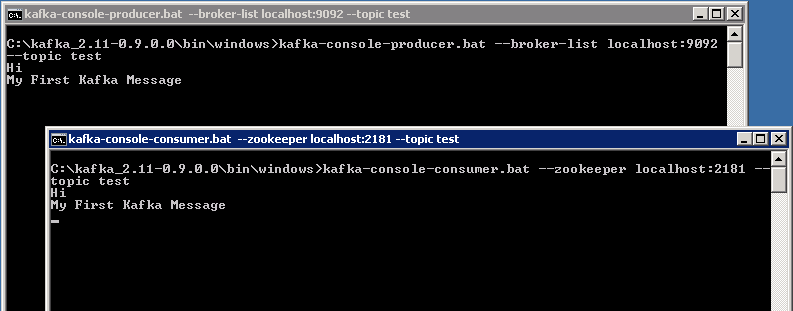
\includegraphics[scale=0.8]{10}  
	\caption[Gambar \textit{consumer}-\textit{producer}]{\textit{consumer}-\textit{producer}} 
	\label{fig:topic-run} 
\end{figure}


\section{Studi Eksplorasi}
\subsection{Eksplorasi Spark Streaming dengan TCP Socket}
Studi Eksplorasi dilakukan dengan mencoba mengumpulkan data dari salah satu penyedia data yaitu TCP Socket. karena ini berupa simulasi, maka file input data web logs akan diunduh terlebih dahulu disimpan pada sebuah file \texttt{accesslog.txt}. Lalu menggunakan perintah \texttt{ ncat -lk 9999 < accesslog.txt} yang artinya \texttt{ncat} akan memasukan data ke TCP port 9999 satu demi satu seolah-olah data yang masuk berupa aliran data.

\begin{figure}[H] 
	\centering  
	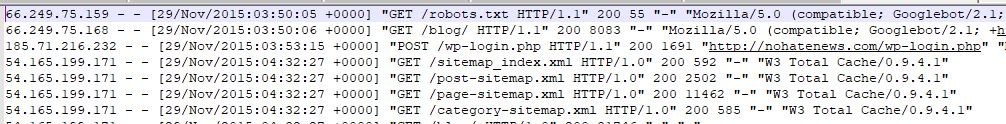
\includegraphics[scale=0.8]{ncatinput}  
	\caption[Gambar File input]{File input} 
	\label{fig:Output-Log-Parser} 
\end{figure}

Data yang akan dianalisis adalah simulasi web logs data stream yang datang dari aktivitas suatu website. Eksplorasi ini akan menghitung seberapa sering suatu file dibuka oleh pengguna. Berikut
cara membuat spark streaming. Contoh Gambar
  
\begin{figure}[H] 
	\centering  
	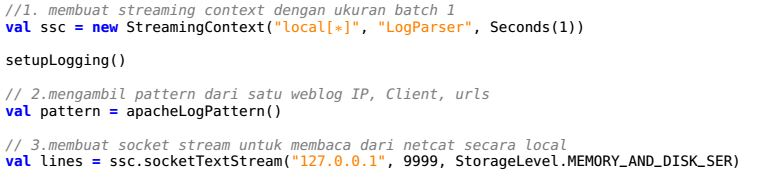
\includegraphics[scale=0.7]{urlcountersetup}  
	\caption[Gambar pengaturan spark streaming]{pengaturan spark streaming} 
	\label{fig:Output-Log-Parser} 
\end{figure}

\begin{figure}[H] 
	\centering  
	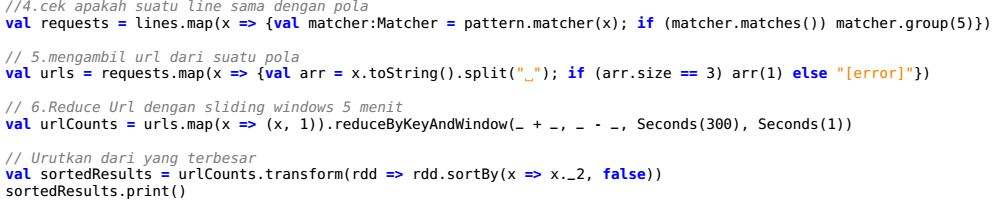
\includegraphics[scale=0.7]{urlcountertransform}  
	\caption[Gambar perhitungan url]{perhitungan url} 
	\label{fig:Output-Log-Parser} 
\end{figure}

Spark streaming dibuat dengan menentukan ukuran batch interval (Streaming Context) selama 1 detik. Pada interval 1 detik Spark Streaming akan mengambil data yang dihasilkan pada interval teresbut. lalu, menggunakan metode dari library ambil web log yang hanya mengikuti pola saja. Jadi, jika ada data lain yang masuk tapi tidak berbentuk web logs akan diabaikan. Menghubungkan batch inteval dengan socket stream untuk mendapatkan data. Mengambil url file dari potongan web logs tersebut contoh \texttt{apachepb.gif}.Menghitung dengan ReduceByKeyAndWindow artinya hitung berapa banyak jumlah url pada key dan windows yang sama. Terakhir urutkan url dari yang memiliki hit paling banyak dan tampilkan 10 hasil terbaik. Contoh Gambar

\begin{figure}[H] 
	\centering  
	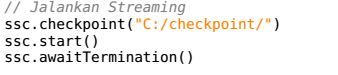
\includegraphics[scale=0.8]{sparkstreamingrun}  
	\caption[Gambar File input]{Menjalankan Spark Streaming} 
	\label{fig:Output-Log-Parser} 
\end{figure}

Terakhir jalankan spark streaming yang telah dibuat. \texttt{ssc.awaitTermination()} menyatakan bahwa proses pengambilan data tidak akan berhenti sampai ada perintah dari user. Contoh Gambar



\begin{figure}[H] 
	\centering  
	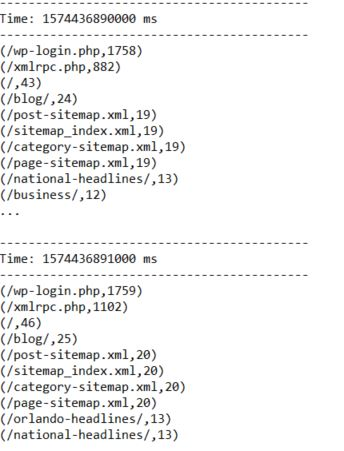
\includegraphics[scale=0.8]{parserOutput}  
	\caption[Gambar Output Web Log]{Output Web log} 
	\label{fig:Output-Log-Parser} 
\end{figure}

hasil dari eksekusi program tersebut adalah batch dengan interval yang telah kita atur dan pada tiap batch interval tersebut berisi hasil komputasi 10 file yang paling sering diakses. Dari hasil dapat disimpulkan pada batch pertama file yang paling sering diakses dalah \texttt{wp-login.php}

\subsection{Eksplorasi dengan Twitter API}
Studi eksplorasi dilakukan dengan mencoba mengumpulkan data dari twitter. Input berupa data stream unggahan tweet dari pengguna twitter di seluruh dunia. Data tidak akan dianalsisis tapi hanya menyimpan status tweet di HDFS. Berikut Langkah-langkah penyimpanan data:

\begin{figure}[H] 
	\centering  
	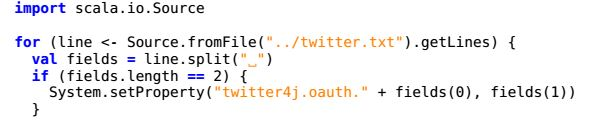
\includegraphics[scale=0.8]{setuptwitter}  
	\caption[Gambar Setup Twitter]{\textit{Setup Twitter}} 
	\label{fig:Output-Twitter} 
\end{figure}

sebelum membuat batch interval harus membuat fungsi yang membaca kredensial twitter dari file \texttt{txt}.

\begin{figure}[H] 
	\centering  
	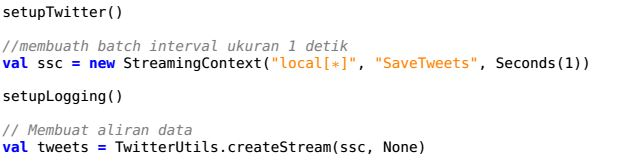
\includegraphics[scale=0.8]{setuptwitterstream}  
	\caption[Gambar Setup Spark Streaming]{\textit{Setup Spark Streaming}} 
	\label{fig:Output-Twitter} 
\end{figure}

langkah pertama adalah mengatur kredensial dari twitter.Lalu membuat batch interval dengan durasi 1 detik. Tetapi, sekarang tidak dihubungkan dengan TCP socket melainkan langsung dari twitter.

\begin{figure}[H] 
	\centering  
	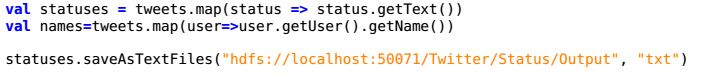
\includegraphics[scale=0.8]{twittertrans}  
	\caption[Gambar transformasi twitter]{transformasi twitter} 
	\label{fig:Output-Twitter} 
\end{figure}

Mengambil tweet object dari aliran data. Transformasi tweets object menjadi status  dan nama user yang artinya hanya isi pesan pengguna dan nama yang diambil. lalu simpan tweet sesuai direktori yang ditentukan dan data akan disimpan dengan format apa. cara menjalankan \textit{Spark Streaming} masih sama dengan TCP Socket.

\begin{figure}[H] 
	\centering  
	\includegraphics[scale=0.6]{outputfolder}  
	\caption[Gambar folder output]{folder outuput} 
	\label{fig:Output-Twitter} 
\end{figure}

\begin{figure}[H] 
	\centering  
	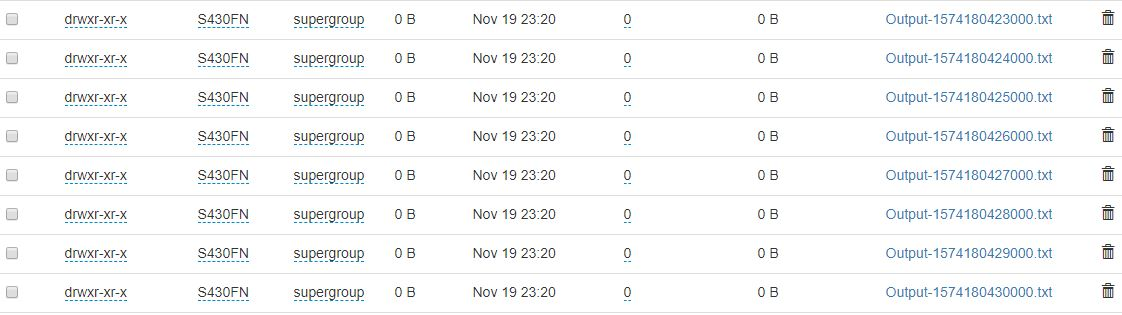
\includegraphics[scale=0.6]{outputfile}  
	\caption[Gambar file output]{file output} 
	\label{fig:Output-Twitter} 
\end{figure}

\begin{figure}[H] 
	\centering  
	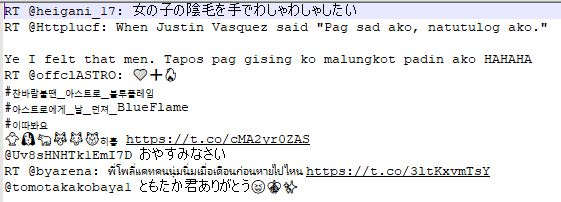
\includegraphics[scale=0.8]{outputtext}  
	\caption[Gambar file output]{isi file} 
	\label{fig:Output-Twitter} 
\end{figure}

Keluaran yang diahsilkan adalah data-data yang dikumpulkan pada interval tertentu. Data dengan interval berbeda akan disimpan di folder yang berbeda juga. Informasi tentang nama user dan status user akan disimpan di file dan folder yang berbeda namun formatnya sama yaitu \texttt{txt}. isi dari file adalah status-status yang diunggah pengguna twitter.

 


 